\documentclass[11pt]{article}

\usepackage[utf8]{inputenc}
\usepackage[T1]{fontenc}
\usepackage{textcomp}
\usepackage{lmodern}
\usepackage{microtype}
\usepackage{graphicx}
\usepackage{booktabs}
\usepackage{array}
\usepackage[margin=1in]{geometry}
\usepackage{amsmath}
\usepackage[numbers]{natbib}
\usepackage{url}
\usepackage{tikz}
\usepackage[hidelinks]{hyperref}

\usetikzlibrary{arrows.meta,positioning}

\title{Governing Interruptions After Deterministic Deterioration Scoring:\\
A Retrospective Evaluation on PhysioNet Challenge 2019}
\author{Satya Venkata Ranga Janaki Sriram Mentey \\
\texttt{srirammentey@ieee.org} \\
ORCID: 0009-0007-2681-006X}
\date{\today}

\begin{document}
\maketitle

\begin{abstract}
\noindent\textbf{Background and Significance:} Clinical deterioration scores and
clinician interruptions are different design objects: a threshold can flag a
concerning state yet still produce repeated or poorly timed interruptions.
Governance applied after deterministic scoring may reduce interruptions without
changing the score.

\noindent\textbf{Objectives:} To compare a frozen dual-lane governance policy on
partial SOFA against threshold-only partial SOFA and against hourly SIRS, NEWS2,
and partial qSOFA, and to attribute the effect to individual mechanisms on a
locked Challenge 2019 holdout.

\noindent\textbf{Materials and Methods:} We replayed Challenge 2019 records
through a deterministic partial-SOFA scorer, tuned governance on
\texttt{training\_setA} ($n=20{,}336$), froze it, and evaluated
\texttt{training\_setB} ($n=20{,}000$) once. Detection counted any governed
emission within $[\texttt{label\_start}-12\,\mathrm{h},\,+6\,\mathrm{h}]$; burden
counted interruptive emissions. We report stay-level bootstrap 95\% CIs
(1{,}000 replicates, seed 42) and drop-one mechanism ablations without
reselection.

\noindent\textbf{Results:} Frozen governed partial SOFA matched threshold-only
sensitivity (79.5\%, 95\% CI 77.0--81.8) while the interruptive lane emitted
13.2\% as many alerts (number needed to alert 106.1, 95\% CI 96.2--116.6).
Incomplete NEWS2 ($\geq 5$) and SIRS ($\geq 2$) reached 76.0\% and 78.5\% but as
ungoverned streams (NNA 163--213); partial qSOFA reached 24.9\%. Removing the
90-minute refractory interval roughly doubled interruptive volume; removing the
page gate raised interruptive sensitivity from 34.0\% to 44.6\%.

\noindent\textbf{Discussion:} Governance shifted retrospective detection onto a
passive lane and confined interruptions, but residual NNA remained high. Results
reflect a proxy label and a partial score.

\noindent\textbf{Conclusion:} Under a frozen setA-to-setB evaluation, governance
reduced page-eligible emissions while retaining retrospective
\texttt{SepsisLabel} detection; this does not establish diagnosis, clinical
benefit, external validity, or superiority to NEWS or qSOFA.
\end{abstract}

\section*{Lay summary}

Hospital early-warning systems often alert clinicians so frequently that
important warnings get lost among routine ones --- a problem called alert
fatigue. We studied whether the \emph{decision to interrupt a clinician} can be
treated as a separate, tunable step that runs after a patient's risk score is
calculated, rather than alerting every time a score crosses a line. Using a
public dataset of intensive-care records, we set the rules on one half of the
data, locked them, and tested them once on the other half. The governed system
flagged the same fraction of deteriorating patients as the raw score (about four
in five) but reduced the number of urgent, interruptive alerts to roughly an
eighth. Two rules did most of the work: a quiet period after each alert, and a
gate that reserved urgent alerts for stronger trajectories. The urgent-alert
count was still high, so this is a starting point, not a finished solution.
Because the data use a proxy definition of illness and an incomplete score,
these results describe alert behaviour only --- not a diagnosis, a clinical
benefit, or readiness for patient care.

\section{Introduction}
\label{sec:intro}

Electronic clinical decision support can generate many technically correct but
operationally weak interruptions. Repeated exposure can reduce responsiveness,
and many interruptive alerts are closed quickly, suggesting that interruption
cost depends on relevance and workflow fit rather than alert count alone
\citep{embi2012,elias2019}. Sepsis-alert trials have also produced mixed
clinical results, reinforcing that a score's discrimination does not by itself
determine the value of the alerting workflow \citep{downing2019}.

Most retrospective deterioration studies treat a positive model or rule output
as the alert. We instead treat scoring and interruption as separate stages. A
deterministic scorer first produces a complete, auditable signal. A shared
governance layer then determines whether the signal should be suppressed, shown
passively, or emitted through an interruptive lane. The governance policy can
use repeated crossings, temporal persistence, baseline-relative change,
refractory windows, and a page gate without changing the underlying clinical
score.

We evaluated this separation using the PhysioNet/Computing in Cardiology
Challenge 2019, which provides hourly ICU records and an onset-aligned
\texttt{SepsisLabel} \citep{reyna2020ccm,reyna2019physionet}. The study asks
one narrow question: can a frozen governance policy reduce page-eligible
emissions relative to threshold-only partial SOFA while retaining retrospective
label detection?

The supported claim is deliberately limited: shared governance reduces
interruptive emissions versus threshold-only partial SOFA while retaining
retrospective Challenge \texttt{SepsisLabel} detection under a frozen
setA-to-setB evaluation. We do not evaluate diagnosis, treatment, mortality,
clinician adoption, MIMIC-IV performance, prospective deployment, or
regulatory readiness.

\section{System}
\label{sec:system}

\subsection{Separation of scoring, governance, and narrative}

The Curie prototype projects clinical events onto a canonical envelope,
transports them through Kafka, and applies versioned deterministic rules in
Apache Flink. The scoring output includes the score, severity, evidence
identifiers, missing components, rule version, and rule-content hash. Shared
governance operates on this deterministic output and assigns passive or
interruptive routing. An optional language-model component may generate a
post-alert narrative, but it cannot create, suppress, escalate, or change an
alert.

\begin{figure}[htbp]
\centering
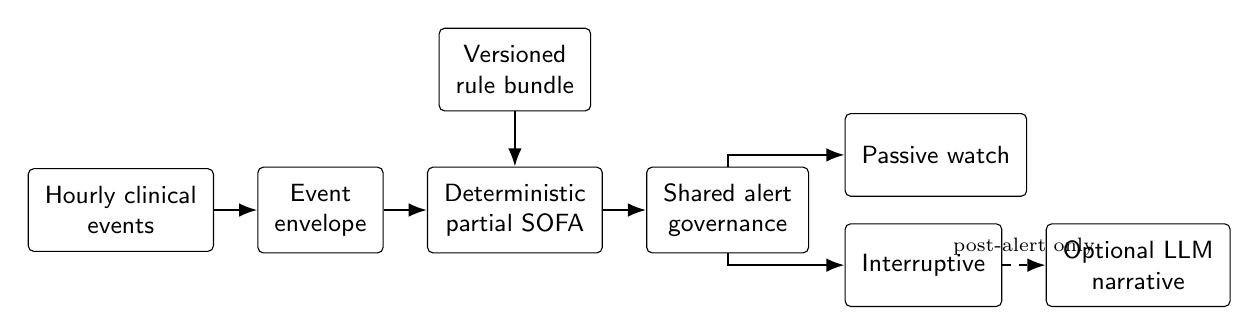
\begin{tikzpicture}[
  font=\small\sffamily,
  box/.style={draw, rounded corners=2pt, align=center, inner sep=6pt, minimum height=1.05cm},
  arr/.style={-{Latex}, thick}
]
\node[box] (a) {Hourly clinical\\events};
\node[box, right=0.55cm of a] (b) {Event\\envelope};
\node[box, right=0.55cm of b] (c) {Deterministic\\partial SOFA};
\node[box, above=0.7cm of c] (r) {Versioned\\rule bundle};
\node[box, right=0.55cm of c] (g) {Shared alert\\governance};
\node[box, right=0.45cm of g, yshift=0.7cm] (w) {Passive watch};
\node[box, right=0.45cm of g, yshift=-0.7cm] (p) {Interruptive};
\node[box, right=0.55cm of p] (l) {Optional LLM\\narrative};
\draw[arr] (a) -- (b);
\draw[arr] (b) -- (c);
\draw[arr] (r) -- (c);
\draw[arr] (c) -- (g);
\draw[arr] (g) |- (w);
\draw[arr] (g) |- (p);
\draw[arr, dashed] (p) -- node[above, font=\scriptsize] {post-alert only} (l);
\end{tikzpicture}
\caption{System boundary used in the retrospective replay. The harness executes
scoring and governance semantics directly. It does not simulate clinician
delivery, acknowledgement, or treatment.}
\label{fig:system}
\end{figure}

\subsection{Governance policy}

The policy family contains five separable mechanisms: (1)~crossings, requiring
repeated qualifying score crossings before selected actions; (2)~persistence,
requiring a qualifying state to persist for a configured duration;
(3)~baseline delta, requiring meaningful change from a recent patient baseline
when enabled; (4)~a refractory interval that suppresses repeated emissions; and
(5)~a page gate that reserves the interruptive lane for stronger trajectories
while preserving a passive watch lane.

The setA-selected configuration used one crossing and no persistence
requirement for the governed watch path, disabled baseline gating, and used a
90-minute refractory interval. Its interruptive page gate required two
crossings, 30 minutes of page-level persistence, a score increase of at least
one point, and at least two positive components.

\section{Methods}
\label{sec:methods}

\subsection{Dataset and study design}

We used PhysioNet Challenge 2019 version 1.0.0. The public resource contains
two training partitions: setA with 20{,}336 stays and setB with 20{,}000 stays
\citep{reyna2020ccm}. Files are licensed under Creative Commons Attribution
4.0 International. We used setA to select and freeze the operating point. We
treated setB as a locked retrospective holdout and did not tune or reselect
policy parameters on it.

This is not an official Challenge submission or an evaluation against the
hidden Challenge test set. \texttt{training\_setB} is a holdout within the
same public challenge resource, not an external hospital validation cohort.

\subsection{Partial SOFA mapping}

SOFA was designed to summarize organ dysfunction across respiratory,
coagulation, liver, cardiovascular, central nervous system, and renal
components \citep{vincent1996sofa}. Challenge records support only a partial
reconstruction. The replay used available oxygenation, mean arterial pressure,
platelet, bilirubin, and creatinine fields with causal forward filling. The
dataset does not provide Glasgow Coma Scale, urine-output windows,
vasopressor-dose ladders, or a reliable mechanical-ventilation flag. We
therefore refer to the result as \textbf{partial SOFA}, not complete SOFA and
not a sepsis diagnosis. Missing inputs were not imputed to reassuring values.
The scorer recorded missing components and required at least two scoreable
components under the frozen study bundle.

\subsection{Comparators and output lanes}

At each hourly update, the same partial-SOFA result fed two paths:
threshold-only partial SOFA (emit whenever the score crossed the configured
alert threshold) and governed partial SOFA (apply the frozen trajectory,
crossing, refractory, and page-gate policy). Governed output was divided into
any governed emission (passive watch plus interruptive; used for detection)
and interruptive emission (urgent or critical page-eligible output; used for
burden and interruptive NNA). ``Interruptive emission'' is an offline routing
decision. It is not an episode-arbitrated page and was not delivered to a
clinician.

Independently of Curie governance, we scored three hourly threshold-only
bedside comparators on the same stays and the same primary window: SIRS
$\geq 2$ using temperature, heart rate, respiratory rate, and white-cell count
\citep{bone1992}; NEWS2 $\geq 5$ (Royal College of Physicians medium trigger)
with consciousness/AVPU scored 0 because it is absent in Challenge 2019
\citep{rcp2017news2}; and partial qSOFA $\geq 2$ using respiratory rate
$\geq 22$ and systolic blood pressure $\leq 100$, with the GCS limb omitted
\citep{seymour2016sepsis3}. These comparators have no refractory window or
page gate. They are not a claim of superiority to NEWS or qSOFA in clinical
practice.

\subsection{Operating-point selection and freeze}

Governance candidates were evaluated on setA. The selected candidate,
\texttt{grid\_p0\_r90\_b0}, was written to the frozen operating-point sidecar
and bound to the resolved study rule bundle. The bundle content hash was
frozen before setB evaluation. The selected setA point had governed
sensitivity of 88.4\% and an interruptive-emission ratio of 0.123 relative to
threshold-only emissions. Named governance profiles plus that frozen winner
are reported as a sparse frontier; that table is not a reconstruction of the
original 23-candidate setA grid.

\subsection{Labels, timing, and outcomes}

For sepsis-positive Challenge records, \texttt{SepsisLabel} becomes positive
at approximately six hours before the Challenge clinical-onset definition
\citep{reyna2020ccm}. We call the first positive label hour
\texttt{label\_start}; we do not call it bedside clinical onset. The primary
timing policy was frozen as \texttt{window\_m12\_p6}: a stay was detected if
any qualifying emission occurred in $[\texttt{label\_start}-12\,\mathrm{h},
\texttt{label\_start}+6\,\mathrm{h}]$. Mean lead time was calculated from the
first governed emission within that bounded window to \texttt{label\_start}.
Grace-0\,h, grace-6\,h, grace-12\,h, early-only, and $\pm 12$\,h definitions
were secondary sensitivity analyses.

Primary holdout metrics were governed sensitivity, interruptive sensitivity,
interruptive NNA (interruptive emissions per interruptive true-positive stay),
and bounded mean lead time. Primary-window 95\% confidence intervals were
stay-level percentile bootstrap intervals (1{,}000 replicates, seed 42). SetB
ablation dropped one frozen mechanism at a time and re-scored setB without
changing the selected winner. Governed false negatives under the primary
window were attributed from replay rows; the committed miss table contains
aggregates only.

\subsection{Engineering checks and other adapters}

Golden fixtures test scorer behavior. Shared fixtures check Python reference
behavior against the Java/Flink implementation. These artifacts are appendix
methods evidence, not an additional results cohort. MIMIC-IV demo, eICU demo,
MIMIC-IV FHIR demo, SYN-ICU, and Synthea adapters exercise the same
adapter-to-harness path. We report no sensitivity, burden, calibration, or
clinical-effect estimate from those sources.

\section{Results}
\label{sec:results}

All numeric tables below are generated from frozen sidecars
(\texttt{make paper-tables}). Do not hand-copy metrics.

\subsection{Selection split}

SetA contained 20{,}336 stays, including 1{,}790 with a positive
\texttt{SepsisLabel}. Under the frozen operating point, threshold-only scoring
emitted 529{,}958 alerts and the interruptive governed lane emitted 64{,}928
alerts (interruptive ratio 0.123). Governed sensitivity was 88.4\%;
interruptive sensitivity was 37.7\%. These are setA selection results. They
are not substituted for the setB primary holdout metrics.

\subsection{Primary setB holdout}

Table~\ref{tab:holdout} reports the frozen setB result under
\texttt{window\_m12\_p6}. The difference between governed and interruptive
sensitivity reflects the intended dual-lane policy: a passive watch can
preserve detection without turning every detection into an interruptive
emission. NNA remains high, indicating that emission reduction alone did not
produce a clinically efficient page stream.

\begin{table}[htbp]
\centering
\footnotesize
\caption{Primary setB holdout results (20{,}000 stays;
\texttt{window\_m12\_p6}). Stay-level percentile bootstrap, 1{,}000
replicates, seed 42. Point estimates match the v1 sidecar.}
\label{tab:holdout}
\begin{tabular}{@{}lccc@{}}
\toprule
Metric & Result & 95\% CI & Interpretation \\
\midrule
Governed sensitivity (\%) & 79.5 & 77.0--81.8 & Any governed emission in-window \\
Interruptive sensitivity (\%) & 34.0 & 31.3--36.8 & Interruptive emission in-window \\
Interruptive NNA & 106.1 & 96.2--116.6 & Interruptive emissions / interruptive TP stay \\
Interruptive / naive emissions & 0.132 & 0.127--0.137 & Page-eligible vs threshold-only SOFA \\
Mean in-window lead (h) & 5.97 & 5.54--6.39 & First governed emission to \texttt{label\_start} \\
\bottomrule
\end{tabular}

\end{table}

\subsection{Timing-definition robustness}

Secondary timing definitions changed absolute sensitivity but produced equal
naive and governed sensitivity for the frozen configuration in each documented
analysis (Table~\ref{tab:robustness}; Figure~\ref{fig:timing}). The 81.1\%
grace-6\,h result is a secondary legacy analysis and must not replace the
primary 79.5\% result.

\begin{table}[htbp]
\centering
\footnotesize
\caption{Secondary setB sensitivity analyses. These modes are not the primary
\texttt{window\_m12\_p6} result.}
\label{tab:robustness}
\begin{tabular}{@{}lcc@{}}
\toprule
Definition & Naive sensitivity (\%) & Governed sensitivity (\%) \\
\midrule
first alert at or before label\_start & 56.3 & 56.3 \\
first alert at or before label\_start + 6 hours & 81.1 & 81.1 \\
first alert at or before label\_start + 12 hours & 84.6 & 84.6 \\
first alert before label\_start & 54.8 & 54.8 \\
any alert in [label\_start - 12 hours, label\_start + 12 hours] & 83.3 & 83.3 \\
\bottomrule
\end{tabular}

\end{table}

\subsection{Bedside comparators}

Table~\ref{tab:comparators} and Figure~\ref{fig:burden} place threshold-only
SIRS, incomplete NEWS2, and partial qSOFA on the same primary window as Curie
lanes. NNA is emissions per in-window true-positive stay for that lane. NEWS2
omits consciousness; qSOFA omits GCS.

\begin{table}[htbp]
\centering
\footnotesize
\caption{SetB threshold-only comparators vs Curie lanes
(\texttt{window\_m12\_p6}). Not a clinical superiority claim.}
\label{tab:comparators}
\begin{tabular}{@{}lccc@{}}
\toprule
Policy & Sensitivity (\%) & Emissions & NNA \\
\midrule
SIRS $\geq$ 2 (Temp, HR, RR, WBC) & 78.5 & 191294 & 213.3 \\
NEWS2 $\geq$ 5 (consciousness omitted) & 76.0 & 141629 & 163.2 \\
Partial qSOFA $\geq$ 2 (RR and SBP; GCS omitted) & 24.9 & 22068 & 77.7 \\
Threshold-only partial SOFA & 79.5 & 311797 & 343.4 \\
Governed partial SOFA (any emit) & 79.5 & 159933 & 176.1 \\
Interruptive governed lane & 34.0 & 41158 & 106.1 \\
\bottomrule
\end{tabular}

\end{table}

\begin{figure}[htbp]
\centering
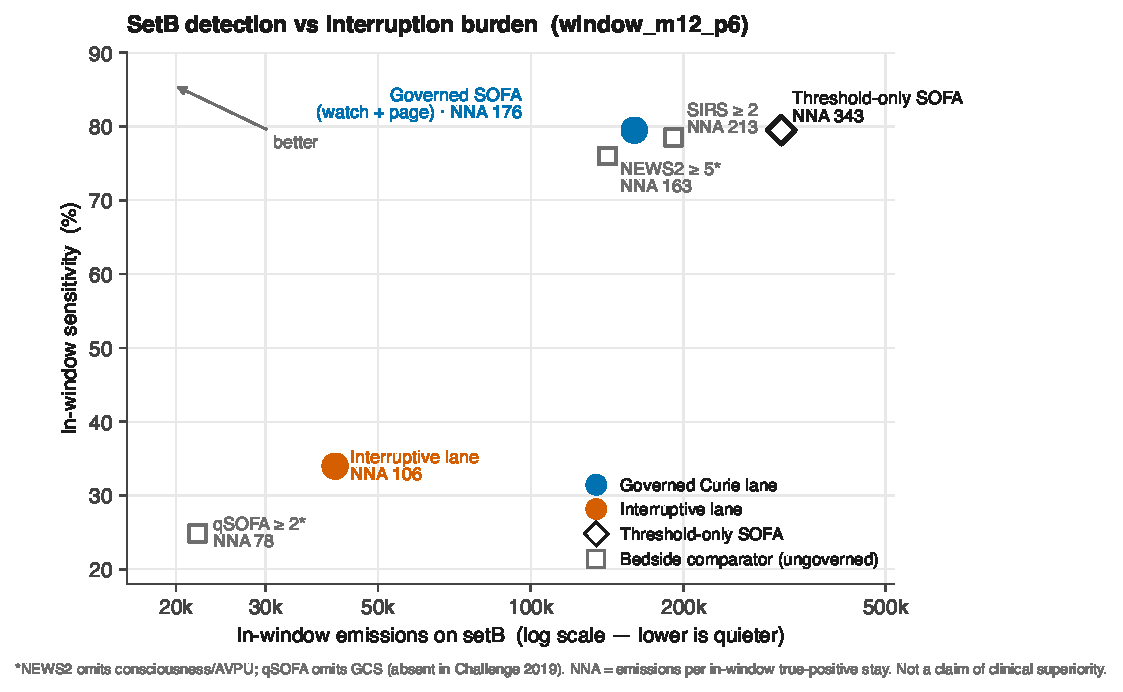
\includegraphics[width=0.92\textwidth]{figures/figure3_detection_burden.pdf}
\caption{SetB detection versus interruption burden under
\texttt{window\_m12\_p6}. NEWS2 omits consciousness/AVPU; qSOFA omits GCS.
NNA is emissions per in-window true-positive stay.}
\label{fig:burden}
\end{figure}

\subsection{SetB ablation of the frozen winner}

Table~\ref{tab:ablation} reports drop-one mechanism evaluations on setB. The
operating point is not reselected. \texttt{drop\_baseline} is a null ablation
(winner already has baseline off). On hourly Challenge spacing, zeroing page
persistence (30\,min) or page crossings ($2\rightarrow 1$) did not change setB
metrics; the 90-minute refractory interval and the page-gate routing decision
did.

\begin{table}[htbp]
\centering
\footnotesize
\setlength{\tabcolsep}{4pt}
\caption{SetB ablation of the frozen winner (\texttt{window\_m12\_p6}). Knobs
are not reselected.}
\label{tab:ablation}
\begin{tabular}{@{}lccccp{3.4cm}@{}}
\toprule
Variant & Gov.\ sens.\ (\%) & Int.\ sens.\ (\%) & Int.\ reduction & Int.\ NNA & Note \\
\midrule
primary\_operating\_point & 79.5 & 34.0 & 0.132 & 106.1 & Frozen winner \\
drop\_baseline & 79.5 & 34.0 & 0.132 & 106.1 & Null (already off) \\
drop\_persistence & 79.5 & 34.0 & 0.132 & 106.1 & No change on hourly rows \\
drop\_crossings & 79.5 & 34.0 & 0.132 & 106.1 & No change on hourly rows \\
drop\_refractory & 79.5 & 36.2 & 0.264 & 199.6 & Watch volume = naive \\
drop\_page\_gate & 79.5 & 44.6 & 0.208 & 127.5 & All emits interruptive \\
\bottomrule
\end{tabular}

\end{table}

\subsection{Miss attribution}

Of 1{,}142 label-positive setB stays, 234 were governed false negatives under
the primary window (Table~\ref{tab:miss}; aggregates only). No in-window
misses were attributed to refractory on the frozen winner: if naive SOFA fired
in-window, a governed emit existed (possibly outside the window).

\begin{table}[htbp]
\centering
\footnotesize
\caption{Governed false negatives on setB under \texttt{window\_m12\_p6}
($n=234$). No stay identifiers.}
\label{tab:miss}
\begin{tabular}{@{}lcc@{}}
\toprule
Reason & Count & Rate (\%) \\
\midrule
Never crossed naive SOFA threshold in-window & 141 & 60.3 \\
Governed emit only outside the window & 58 & 24.8 \\
Never scoreable (missing inputs) & 35 & 15.0 \\
\bottomrule
\end{tabular}

\end{table}

Named profiles plus the frozen winner on setA are in
Table~\ref{tab:pareto}. That figure is not a reconstruction of the original
23-candidate grid.

\begin{table}[htbp]
\centering
\footnotesize
\caption{Named governance profiles plus frozen winner on setA under
\texttt{window\_m12\_p6}.}
\label{tab:pareto}
\begin{tabular}{@{}lcccc@{}}
\toprule
Candidate & Gov.\ sens.\ (\%) & Int.\ reduction & Int.\ sens.\ (\%) & Selected \\
\midrule
strict & 6.8 & 0.024 & 6.8 & no \\
balanced & 12.7 & 0.075 & 12.6 & no \\
sensitive & 87.6 & 0.161 & 38.9 & no \\
accuracy & 87.6 & 0.161 & 38.9 & no \\
dual & 87.6 & 0.123 & 32.5 & no \\
grid\_p0\_r90\_b0 & 87.6 & 0.123 & 32.5 & yes \\
\bottomrule
\end{tabular}

\end{table}

\begin{figure}[htbp]
\centering
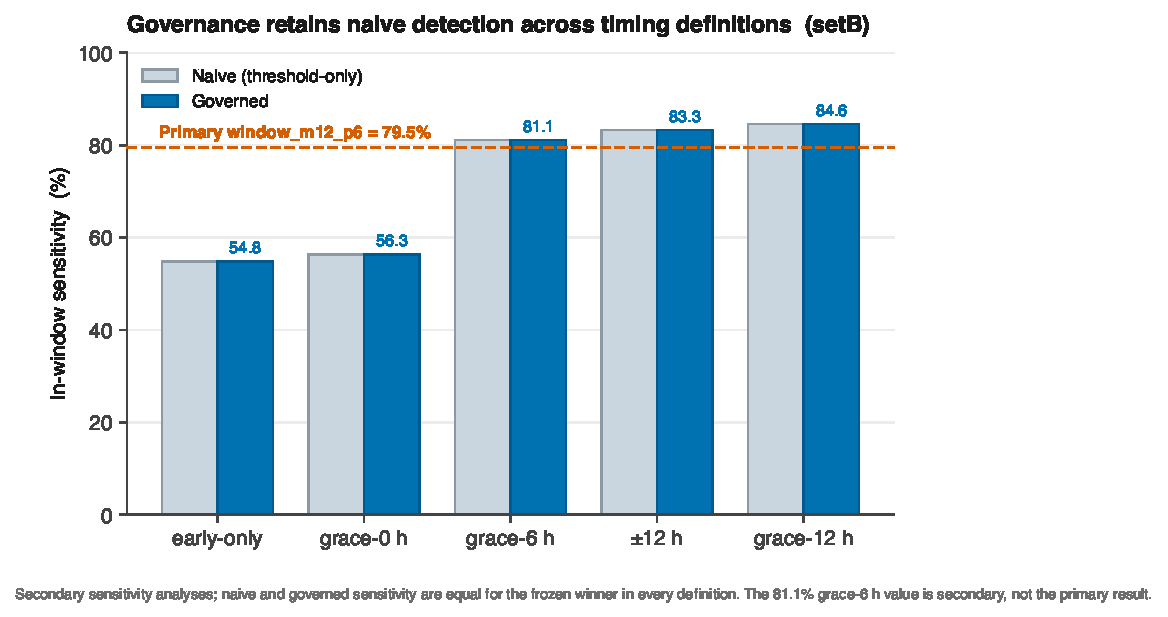
\includegraphics[width=0.92\textwidth]{figures/figure4_timing_robustness.pdf}
\caption{Naive versus governed sensitivity across secondary timing
definitions on setB. The dashed line is the primary
\texttt{window\_m12\_p6} governed sensitivity (79.5\%).}
\label{fig:timing}
\end{figure}

\section{Discussion}
\label{sec:discussion}

This study evaluates the alert policy rather than proposing a new predictive
model. On the setB primary window, incomplete NEWS2 and SIRS approached
governed partial-SOFA sensitivity (76.0\% and 78.5\% vs 79.5\%) but as
ungoverned hourly streams with NNA 163--213. Partial qSOFA was specific and
quiet (24.9\% sensitivity, 22{,}068 emissions) because the GCS limb is
missing. Frozen governance matched naive SOFA detection at 79.5\% while the
interruptive lane retained 13.2\% of naive SOFA volume. Ablation shows that
the 90-minute refractory interval is what keeps watch volume below naive SOFA,
and that the page gate---not page persist or page crossings on hourly
rows---is what holds interruptive sensitivity at 34.0\% rather than 44.6\%.

The result supports dual-lane design: retrospective detection can be
represented passively while a more selective policy controls interruption. It
does not show that the interruptive lane is already optimal. An interruptive
NNA of 106.1 is a substantial residual burden and should be treated as a
design target. The comparison to SIRS/NEWS2/qSOFA is a Challenge-2019
detection/burden plane, not evidence that Curie outperforms those scores in
clinical practice.

Threshold-only comparisons often collapse model output, user-interface
behavior, and clinician workflow into one binary alert. The present design
makes those layers explicit. Persistence, crossings, refractory windows, and
page gating can be studied as versioned policy parameters while the clinical
score remains unchanged.

The next evidence step is not to treat unlabeled demo datasets as external
validation. A separate study should execute a pre-specified MIMIC-IV protocol
using availability-time replay, a full or explicitly partial SOFA
reconstruction, Sepsis-3-aligned labels, and subgroup analysis. A later silent
prospective study would be required to measure delivered alert burden,
clinician response, workflow fit, safety, and patient outcomes.

\section{Limitations}
\label{sec:limitations}

First, Challenge \texttt{SepsisLabel} is an onset-aligned proxy derived for a
prediction competition. It is not prospective bedside adjudication, and it
begins approximately six hours before the Challenge clinical-onset definition.
Reported lead time is therefore relative to \texttt{label\_start}, not proof
of six hours of actionable clinical warning.

Second, the score is partial SOFA. Challenge data omit GCS, urine output
windows, vasopressor dose ladders, and reliable mechanical-ventilation
context.

Third, setB is a holdout within one public challenge, not an external clinical
cohort. The study does not estimate transportability, site calibration,
distribution shift, subgroup fairness, or prospective performance.

Fourth, interruptive outputs are emission-level page candidates. They were
not episode arbitrated, delivered, or reviewed by clinicians. NNA therefore
measures retrospective emissions per detected positive stay, not pages
required for a useful clinical action.

Finally, fixture and demo-schema checks prove implementation behavior only.
They do not provide a second clinical cohort.

\section{Claim boundary}
\label{sec:claims}

This manuscript supports a retrospective alert-governance claim on PhysioNet
Challenge 2019. It does not support any statement that Curie diagnoses sepsis;
improves mortality, organ failure, treatment time, or length of stay; works on
MIMIC-IV, eICU, FHIR demo, SYN-ICU, Synthea, or a hospital feed; is clinically
validated, production-ready, FDA-cleared, or suitable for patient care; or
outperforms a clinical score, commercial product, or deployed workflow.

\section{Reproducibility}
\label{sec:repro}

Tables regenerate with \texttt{make paper-tables}. The supplementary
reproducibility package rebuilds with \texttt{make manuscript}. The freeze
checklist and sidecar pins are in this directory's reproducibility note.
Patient-level source files remain outside version control.

\section*{Data and code availability}

The PhysioNet/Computing in Cardiology Challenge 2019 dataset version 1.0.0 is
publicly available from PhysioNet under the Creative Commons Attribution 4.0
International license. Patient-level source files and replay outputs are not
redistributed. All frozen operating points, timing policies, resolved rule
bundles, comparator, ablation, miss-attribution, and bootstrap sidecars, content
hashes, and the reproducibility manifest are included in the project repository;
every table regenerates with \texttt{make paper-tables} and the supplementary
reproducibility package with \texttt{make manuscript}.

\section*{Ethics approval}

This study used only the publicly available, fully de-identified
PhysioNet/Computing in Cardiology Challenge 2019 dataset and involved no new
human-subjects data collection; institutional review board approval was
therefore not required.
% AUTHOR: confirm this wording against your institution's policy before submission.

\section*{Funding}

This research received no external funding and was conducted by the author on a
self-funded basis.

\section*{Competing interests}

The author declares no competing interests.

\section*{Acknowledgements}

% AUTHOR: add acknowledgements (data providers, colleagues, compute), or delete
% this section.

\bibliographystyle{unsrtnat}
\bibliography{references}

\end{document}
